
% \subsection{Setup}
% \begin{figure}
%   \centering
%   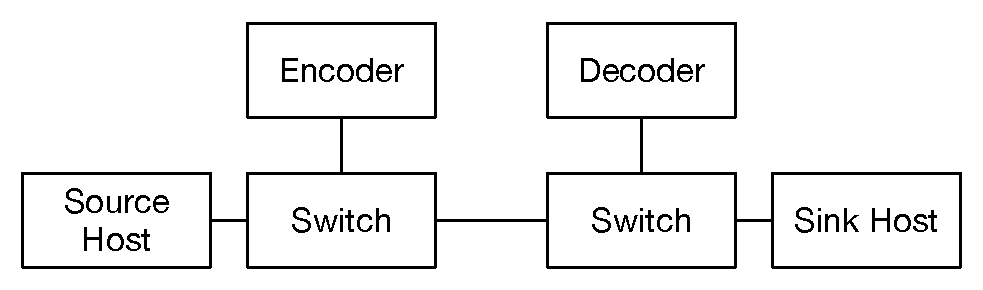
\includegraphics[width=0.3\paperwidth]{exp_topo.pdf}
%   \caption{\label{fig:exp_topo} Testbed topology for benchmarks.}
% \end{figure}

% Figure~\ref{fig:exp_topo} depicts the testbed we used to benchmark \OurSys.
% \hg{This setup was not used to test the FPGA, so it probably does not
% belong in a section on its own.}
% The two traffic generation hosts are each connected to different \OurSys
% enabled switches, which are themselves connected by a 10 GbE link. The
% switches are Wedge BF32-100X's with Barefoot Tofino~\cite{tofino} P4 
% programmable forwarding engines. \lei{TODO: fix cite}


To measure the effect of faulty links and \OurSys at the protocol and
application level, we developed a P4 pipeline for the Barefoot Tofino that
models the behavior of faulty links and FEC in real-time.
Figure~\ref{fig:p4ModelTopo} illustrates the pipeline.



% of the encoder,  decoder, and
% faulty link, and can be reconfigured with different FEC and  packet loss
% parameters at runtime via the control plane.

The \textbf{encoder model} adds the \OurSys header to packets egressing on
the faulty link and generates blank parity packets. 

%It tracks per-port block IDs and  packet indices using P4 register
%arrays. To generate parity packets, the  model clones the last data packet in
%each block with the Tofino's multicast engine.

The \textbf{faulty link model} adds a \emph{corruption header} to each packet
egressing the faulty link, indicating whether the next switch should
consider the packet lost. It uses the Tofino's  random number generator to
select packets for loss according to a binomial  distribution.


Finally, the \textbf{decoder model} processes packets ingressing from the
faulty link. It removes added headers and passes non- corrupt packets to
forwarding. It withholds corrupt packets, using recirculation, until the block
ends. If it has counted at least $K$ data plus parity packets in the block,
the model "recovers" the corrupt packets by allowing them to pass to
forwarding; else, the model drops them.

We deployed the model in the testbed network shown in
Figure~\ref{fig:p4ModelTopo} and ran 10-second TCP file transfers from
the client to the server using Iperf with different settings for $k$, $h$, and
loss rate. 

%We ran 25 trials for each configuration.



% \begin{figure}
%   \centering
%   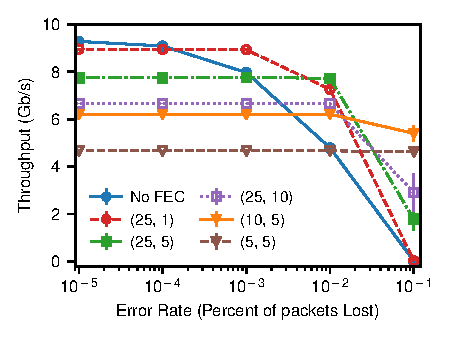
\includegraphics[width=0.3\paperwidth]{figures/lossVsTput.pdf}
%   \caption{\label{fig:lossVsTput} Iperf throughput at different loss rates.}
% \end{figure}

% \begin{figure}
%   \centering
%   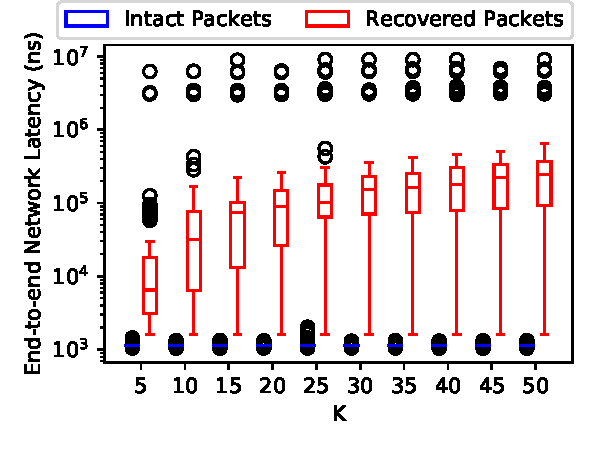
\includegraphics[width=0.3\paperwidth]{figures/udpLatency.pdf}
%   \caption{\label{fig:lossVsLatencyUdp} Network latency for a 100 Mb/s UDP flow (H = 5, loss rate = $10 ^{-2}$).}
% \end{figure}

% \begin{figure}
%   \centering
%   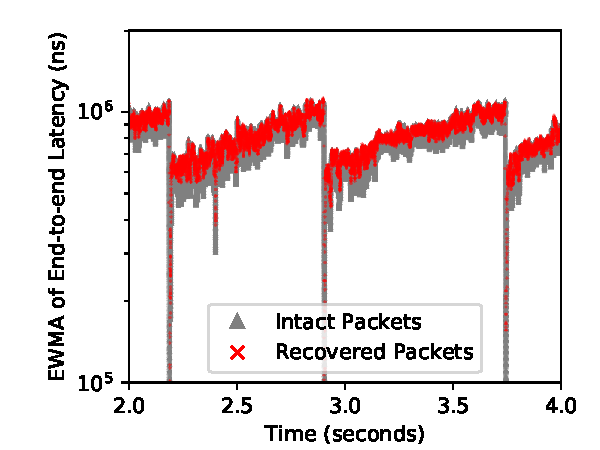
\includegraphics[width=0.3\paperwidth]{figures/tcpLatency.pdf}
%   \caption{\label{fig:lossVsLatencyTcp} Network latency for a 9 Gb/s TCP flow (K = 25, H = 5, loss rate = $10 ^{-2}$).}
% \end{figure}


%Congestion window size ($cwnd$) determines how much data the sender 
%can transmit before receiving an ACK, limiting the transmission rate 
%to approximately $cwnd$ * round trip time.
%TCP increases $cwnd$ linearly 
%with successful packet deliveries, and reduces it exponentially upon 
%packet loss.


Figure~\ref{fig:lossVsTput} shows TCP throughput with different FEC
configurations as loss rate varied. With \OurSys, Iperf sustained  over 5 Gb/s
with loss up to $10^{-1}$ (1 out of every 10 packets dropped). Without
\OurSys, Iperf's throughput at that loss rate was under 25 Mb/s. 

Figure~\ref{fig:lossVsWindow} shows average congestion window size ($cwnd$) in the
trials. Random packet loss at rates higher than $10^{-5}$ caused TCP to
reduce $cwnd$ significantly, resulting in the throughput drop in
Figure~\ref{fig:lossVsTput}. With FEC, $cwnd$ remains high as
loss rate increases, especially when using high levels of redundancy, e.g.,
$(k, h) = (5, 5)$.

Figure~\ref{fig:latency} shows end-to-end network latency. Latency increased
with $h/k$ because of the dynamics between the FEC model and TCP. The TCP
source under-estimated its contribution to congestion because it was unaware
of congestion related drops of parity packets. This caused high average queue
depths in the egress to the faulty link, e.g., up to 1 MB for $(5,5)$, and
therefore high latency. A solution that requires no modification to TCP is
rate limiting entry to the encoder based on the effective capacity of the
faulty link, given $h$, $k$ and the loss rate. This would drop data packets
before parity packet generation to ensure that TCP senders are aware of  all
drops relating to their flows. We tested our hypothesis by repeating the $(5,
5)$ trials with the sending host limited to 4.5 Gb/s, just under effective
capacity. The average latency was 41 $\mu$s, within the same range as latency
in the no FEC trials. We plan to integrate rate limiting into the next
versions of \OurSys and the P4 models, using the metering features of P4 and
the Tofino.

% Figure~\ref{fig:latency} shows end-to-end network latency. Latency increased
% with $h/k$ because of the dynamics between the FEC model and TCP. The TCP
% source under-estimated its contribution to congestion because it was unaware
% of parity packet drops relating to its flow. This caused high average queue
% depths in the egress to the faulty link, e.g., up to 1 MB for $(5,5)$, which
% increased latency. A solution that requires no modification to TCP is rate
% limiting entry to the encoder based on the effective capacity of the faulty
% link, given $h$, $k$ and the loss rate. This would drop data packets before
% parity packet generation to ensure that TCP senders are aware of  all drops
% relating to their flows. We tested our hypothesis by repeating the $(5, 5)$
% trials with the sending host limited to 4.5 Gb/s, just under effective
% capacity. The average latency was 41 $\mu$s, within the same range as latency
% in the no FEC trials. We plan to integrate rate limiting into the next
% versions of \OurSys and the P4 models, using the metering features of P4 and
% the Tofino.

% As Figure~\ref{fig:latency} shows, the model suggests that FEC may add
% latency. The root cause lies in the dynamics between the FEC model and TCP.
% The TCP source under-estimated its contribution to congestion because it was
% unaware of parity packet drops relating to its flow. This caused congestion in
% the egress to the faulty link, e.g., with queue depths of up to 1 MB for
% $(5,5)$, which increased latency. A solution that requires no modification to
% TCP is rate limiting entry to the encoder based on the effective capacity of
% the faulty link, given $h$, $k$ and the loss rate. This would ensure that the
% TCP sender was aware of all drops related to its flow so it could correctly
% estimate its contribution to congestion. We tested our hypothesis by repeating
% the $(5, 5)$ trials with the sending host limited to 4.5 Gb/s, just under
% effective capacity. The average latency was only 41 $\mu$s, within the same
% range as latency in the no FEC trials. We plan to integrate rate limiting into
% the next versions of \OurSys and the P4 models, using the metering features of
% P4 and the Tofino.

% , support rate limiting in their
% % traffic  managers that can be dynamically adjusted at runtime.




% in-network latency, i.e., from the  ingress
% pipeline of the encoding switch to the egress pipeline of the  decoding
% switch, in trials with no loss. FEC added under 1ms of average latency in  all
% trials. Latency was proportional to $h/k$, because the parity packets
% increased the average length of the egress queue to the faulty port by
% approximately that factor. TCP adjusts to higher latency  by increasing
% $cwnd$, which explains why $cwnd$ increases with ($h/k$) in
% Figure~\ref{fig:lossVsWindow}.



% % This figure shows the impact of H. 

% Figure~\ref{fig:lossVsTput} also shows the bandwidth overhead of  FEC, which
% is dominated by the number of parity packets per block ($H$).  At loss rates
% greater than or equal to $10^{-4}$ the bandwidth overhead of adding  parity
% packets had less of an impact on TCP throughput than lost packets, for  most
% configurations tested. To reduce bandwidth overhead, the FEC  can be tuned for the
% loss rate of each specific link, which is reportedly stable over
% time~\cite{corropt}.



% % This figure shows the impact of K.

% To understand how FEC impacts latency, we measured the latency  between the
% ingress pipeline from the source server and the egress pipeline  to the sink
% server, using the nanosecond precision  timestamps of the Tofino, with packets
% routed back through the first  switch before egressing to the sink.
% Figure~\ref{fig:lossVsLatencyUdp}  plots an EWMA of latency for packets in a
% 100 Mb/s UDP flow. For  intact packets, latency was low because they did not
% invoke  the decoder. For  recovered packets, however, the decoder increased
% latency. Average  latency increased with block size because  recovery requires
% the decoder to wait until all the parity packets  for a block arrive. The
% maximum observed latency for recovered packets  was high, around 9 MS. This
% was due to the behavior of the iperf  UDP generator, which periodically paused
% for up to 9 MS between  sending packets, to meet the 100 Mb/s target. The high
% inter-packet  arrival time stalled the generation of parity packets and thus
% the  recovery of any lost packets in the same block.
% \lei{\#Shrink Candidate\#}

% Figure~\ref{fig:lossVsLatencyTcp} plots a time series of latency EWMA  for TCP
% packets in a single maximum rate flow (around 9 Gb/s). The difference in
% latency between recovered versus intact packets was almost indistinguishable.
% Latency for all packets was not dominated by the decoder, but instead by time
% spent  in egress buffers in the switch, which repeatedly filled due to TCPs
% congestion  control dynamics, i.e., causing the familiar ``sawtooth'' pattern
% in Figure~\ref{fig:lossVsLatencyTcp}. Additionally, the latency for packet
% recovery was lower with the TCP workload because average packet rate was
% around 1 order of magnitude higher.



